% !TeX root = construct.tex

\chapter{Are Triangles with the Equal Area and Perimeter Congruent?}\label{c.congruent}

Are triangles with the equal area and equal perimeter congruent? Not necessarily: the triangles with sides $(17,25,28)$ and $(20,21,27)$ both have perimeter $70$ and area $210$. Barabash \cite{marita} shows that given a equilateral triangle, there are non-congruent triangles with the same area and perimeter; however, her proof is not constructive. This document (based on [2]) shows that given a triangle with rational sides, it is possible to construct a non-congruent triangle with \emph{rational} sides and the same area and perimeter.

As a bonus, an elegant proof of Heron's formula is obtained.

\vspace{-2ex}

\section{From triangles to elliptic curves}

The following diagram shows $O$, the \emph{incenter} of an arbitrary triangle $\triangle ABC$, which is the intersection of the bisectors of the three angles.  Drop altitudes from $O$ to the sides. The altitudes have length $r$, the raidus of the inscribed circle. The altitudes and angle bisectors create three pairs of congruent \emph{right} triangles:
\[
\triangle AOB'\cong \triangle AOC',\quad \triangle BOA'\cong \triangle BOC',\quad \triangle COA'\cong \triangle COB'\,.
\]

\vspace*{-6ex}

\begin{center}
\begin{tikzpicture}[baseline=-6mm,scale=1.8]
% Draw base and path two lines at known angles
\draw (0,0) coordinate (a) node[xshift=-6pt] {$A$} -- (0:6) coordinate (b) node[xshift=6pt] {$B$};
\path[name path=ac] (a) -- +(50:4);
\path[name path=bc] (b) -- +(150:5);
% Get their intersection and draw lines between vertices
\path[name intersections={of=ac and bc,by=c}];
\node[above] at (c) {$C$};
\draw (a) -- (c) -- (b) -- (a);
% Label angles with tick marks
\draw (a) ++(0:5mm) arc (0:50:5mm);
\draw (a) ++(10:4.5mm) -- +(10:1mm);
\draw (a) ++(15:4.5mm) -- +(15:1mm);
\draw (a) ++(35:4.5mm) -- +(35:1mm);
\draw (a) ++(40:4.5mm) -- +(45:1mm);
\draw (b) ++(150:7mm) arc (150:180:7mm);
\draw (b) ++(157.5:6.5mm) -- +(157.5:1mm);
\draw (b) ++(172.5:6.5mm) -- +(172.5:1mm);
\draw (c) ++(230:5mm) arc (230:330:5mm);
\draw (c) ++(250:4.5mm) -- +(250:1mm);
\draw (c) ++(255:4.5mm) -- +(255:1mm);
\draw (c) ++(260:4.5mm) -- +(260:1mm);
\draw (c) ++(300:4.5mm) -- +(300:1mm);
\draw (c) ++(305:4.5mm) -- +(305:1mm);
\draw (c) ++(310:4.5mm) -- +(310:1mm);
% Path bisectors of two lines
\path[name path=bia] (a) -- +(25:3.5);
\path[name path=bib] (b) -- +(165:5);
% Intersection of angle bisectors
\path [name intersections={of=bia and bib,by=center}];
% Draw angle bisectors to center
\draw (a) -- (center);
\draw (c) -- (center);
\draw (b) -- (center);
% Draw radii
\draw (center) -- node[left] {$r$} ($(a)!(center)!(b)$) node[below,yshift=-2pt] {$C'$} coordinate (ap);
\draw (center) -- node[left,yshift=-4pt] {$r$} ($(a)!(center)!(c)$) node[above left] {$B'$} coordinate (bp);
\draw (center) -- node[right] {$r$} ($(b)!(center)!(c)$) node[above right] {$A'$} coordinate (cp);
% Draw dots
\fill (center) circle (1pt) node[right,xshift=4pt,yshift=4pt] {$O$};
\fill (a) circle (1pt);
\fill (b) circle (1pt);
\fill (c) circle (1pt);
\fill (ap) circle (1pt);
\fill (bp) circle (1pt);
\fill (cp) circle (1pt);
% Draw right angle squares
\draw (ap) -- ++(90:4pt) -- ++(0:4pt) -- ++(-90:4pt);
\draw (bp) -- ++(-40:4pt) -- ++(-130:4pt) -- ++(-220:4pt);
\draw (cp) -- ++(-30:4pt) -- ++(-120:4pt) -- ++(-210:4pt);
\end{tikzpicture}
\end{center}

\vspace*{-3ex}


The following diagram shows the sides $a,b,c$ divided into segments $u,v,w$, and the angles $\alpha/2,\beta/2,\gamma/2$:

\vspace*{-3ex}

\begin{center}
\begin{tikzpicture}[baseline=-6mm,scale=1.8]
% Draw base and path two lines at known angles
\draw (0,0) coordinate (a) node[xshift=-8pt] {$A$} -- (0:6) coordinate (b) node[xshift=6pt] {$B$};
\path[name path=ac] (a) -- +(50:4);
\path[name path=bc] (b) -- +(150:5);
% Get their intersection and draw lines between vertices
\path[name intersections={of=ac and bc,by=c}];
\node[above] at (c) {$C$};
\draw (a) -- node[right] {$b$} (c) -- node[below] {$a$} (b) -- node[above] {$c$} (a);
% Path bisectors of two lines
\path[name path=bia] (a) -- +(25:3.5);
\path[name path=bib] (b) -- +(165:5);
% Intersection of angle bisectors
\path [name intersections={of=bia and bib,by=center}];
% Draw angle bisectors to center
\draw (a) -- (center);
\draw (c) -- (center);
\draw (b) -- (center);
% Labels of angles
\node[above,xshift=5pt,yshift=21pt] at (center) {$\gamma/2$};
\node[above left,xshift=-4pt,yshift=21pt] at (center) {$\gamma/2$};
\node[above right,xshift=4pt,yshift=-5pt] at (center) {$\beta/2$};
\node[below right,yshift=-6pt] at (center) {$\beta/2$};
\node[left,xshift=-8pt,yshift=3pt] at (center) {$\alpha/2$};
\node[below left,xshift=2pt,yshift=-6pt] at (center) {$\alpha/2$};
% Draw radii
\draw (center) -- node[near end,left] {$r$} ($(a)!(center)!(b)$) coordinate (cp) node[below,yshift=-2pt] {$C'$};
\draw (center) -- node[left,near end,yshift=-4pt] {$r$} ($(a)!(center)!(c)$) coordinate (bp) node[above left] {$B'$};
\draw (center) -- node[right,near end] {$r$} ($(b)!(center)!(c)$) coordinate (ap) node[above right] {$A'$};
\fill (ap) circle (1pt);
\fill (bp) circle (1pt);
\fill (cp) circle (1pt);
\fill (a) circle (1pt);
\fill (b) circle (1pt);
\fill (c) circle (1pt);
% Draw dot at center
\fill (center) circle (1pt);
% Labels of line segments
\path (a) -- node[below,yshift=-2pt] {$u$} (cp);
\path (a) -- node[left,xshift=-2pt]  {$u$} (bp);
\path (b) -- node[below,yshift=-2pt] {$v$} (cp);
\path (b) -- node[above,xshift=2pt] {$v$} (ap);
\path (c) -- node[above,xshift=-2pt] {$w$} (bp);
\path (c) -- node[above,xshift=2pt] {$w$} (ap);
\end{tikzpicture}
\end{center}

The area of $\triangle ABC$ is the sum of the areas of $\triangle AOC, \triangle BOC, \triangle AOB$:
\begin{equation}
A = \frac{1}{2}(w+v)r + \frac{1}{2}(v+u)r + \frac{1}{2}(u+w)r = \frac{1}{2}\cdot 2(u+v+w)r = rs\,, \label{eq.area1}
\end{equation}
where the semi-perimeter is: $s=u+v+w$. The lengths of $u,v,w$ can be computed from the angles and $r$:
\erh{12pt}
\begin{equationarray}{rlc}
\tan \frac{\alpha}{2} &=& \frac{u}{r}\label{eq.alpha}\\
\tan \frac{\beta}{2} &=& \frac{v}{r}\label{eq.beta}\\
\tan \frac{\gamma}{2} &=& \frac{w}{r}\label{eq.gamma}\,.
\end{equationarray}
$s$ can now be expressed in terms of the tangents:
\[
s = u+v+w = r\tan \frac{\alpha}{2}+r\tan \frac{\beta}{2}+r\tan \frac{\gamma}{2} = r\left(\tan \frac{\alpha}{2}+\tan \frac{\beta}{2}+\tan \frac{\gamma}{2}\right)\,,
\]
and by Equation~\ref{eq.area1} the area is:
\begin{equation}
A = rs = r^2\left(\tan \frac{\alpha}{2}+\tan \frac{\beta}{2}+\tan \frac{\gamma}{2}\right)\,.\label{eq.area2}
\end{equation}
From $A=rs$ we have $r=A/s$, so Equation~\ref{eq.area2} can be written as:
\begin{equation}
\tan \frac{\alpha}{2}+\tan \frac{\beta}{2}+\tan \frac{\gamma}{2} = \frac{A}{r^2} = \frac{A}{(A/s)^2} = \frac{s^2}{A}\,.\label{eq.area3}
\end{equation}
Since the sum of the angles $\alpha,\beta,\gamma$ is $2\pi$:
\begin{eqnarray}
%\gamma &=& 2\pi - (\alpha + \beta)\\
\gamma/2 &=& \pi - (\alpha/2 + \beta/2)\\
\tan\gamma/2 &=& \tan(\pi - (\alpha/2 + \beta/2))\\
 &=& -\tan (\alpha/2 + \beta/2)\\
&=& \frac{\tan\alpha/2 + \tan\beta/2}{\tan\alpha/2 \, \tan\beta/2-1}\,.\label{eq.tangent1}
\end{eqnarray}
Here is proof of the formula for the tangent of the sum of two angles:
\begin{eqnarray}
\tan (\theta+\phi) &=& \frac{\sin(\theta+\phi)}{\cos(\theta+\phi)}\\
&=&\frac{\sin\theta\cos\phi+\cos\theta\sin\phi}{\cos\theta\cos\phi-\sin\theta\sin\phi}\\
%\tan (\theta+\phi) &=&\frac{\displaystyle\frac{\sin\theta}{\cos\theta}+\frac{\sin\phi}{\cos\phi}}{\displaystyle 1-\frac{\sin\theta\sin\phi}{\cos\theta\cos\phi}}\label{eq.tangent2}\\
&=&\frac{\tan\theta + \tan \phi}{1-\tan\theta\tan\phi}\,,\label{eq.tangent3}
\end{eqnarray}
where Equation~\ref{eq.tangent3} is obtained by dividing by $\cos\theta\cos\phi$.

\newpage

Let us simplify the notation by defining variables for the tangents:

\vspace{-4ex}

\erh{12pt}
\begin{equationarray*}{rcl}
x&=&\tan \frac{\alpha}{2}\\
y&=&\tan \frac{\beta}{2}\\
z&=&\tan \frac{\gamma}{2}\,.
\end{equationarray*}
By Equation~\ref{eq.tangent1} we can replace $z=\tan\gamma/2$ by an expression in $x,y$:
\begin{equation}
z = \frac{x+y}{xy-1}\,.\label{eq.xy1}
\end{equation}
With this notation, Equation~\ref{eq.area3} becomes:
\begin{equation}
x+y+\frac{x+y}{xy-1}=\frac{s^2}{A}\,.\label{eq.xy2}
\end{equation}
Given fixed values of $A$ and $s$, are there multiple solutions to Equation~\ref{eq.xy2}?

For the right triangle $(3,4,5)$:
\begin{equation}
\frac{s^2}{A} = \frac{\left(\frac{1}{2}(3+4+5)\right)^2}{\frac{1}{2}\cdot 3\cdot 4} = \frac{6^2}{6}=6\,.
\end{equation}
If there is another solution Equation~\ref{eq.xy2}, it can be written as:
\begin{equation}
x^2y + xy^2 -6xy + 6 = 0\,.\label{eq.elliptic}
\end{equation}
This is an equation for an \emph{elliptic curve}. Elliptic curves were used by Andrew Wiles' in his proof of Fermat's last theorem. They have also been used in public-key cryptography.

\section{Solving the equation for the elliptic curve}

A portion of the graph of Equation~\ref{eq.elliptic} is shown in the diagram below. Any point on the closed curve in the first quadrant is a solution to the equation because the lengths of the sides of the triangle must be positive. $A,B,D$ correspond to the triangle $(3,4,5)$ as we shall show below. To find additional (\emph{rational}) solutions, the \emph{method of two secants} is used.\footnote{McCallum [2] notes that there are an infinite number of rational solutions.}

Draw a secant through the points $A=(2,3)$ and $B=(1,2)$. It intersects the curve at $C=(-1.5,-0.5)$, but this does not give a solution because the values are negative. If we draw a second secant from $C$ to $D=(3,2)$, the intersection with the curve at $E$ does give a new solution.\footnote{$(1.5,1.2)$ is an approximation displayed by GeoGebra. We will compute the exact coordinates of $E$ below.}

\begin{center}
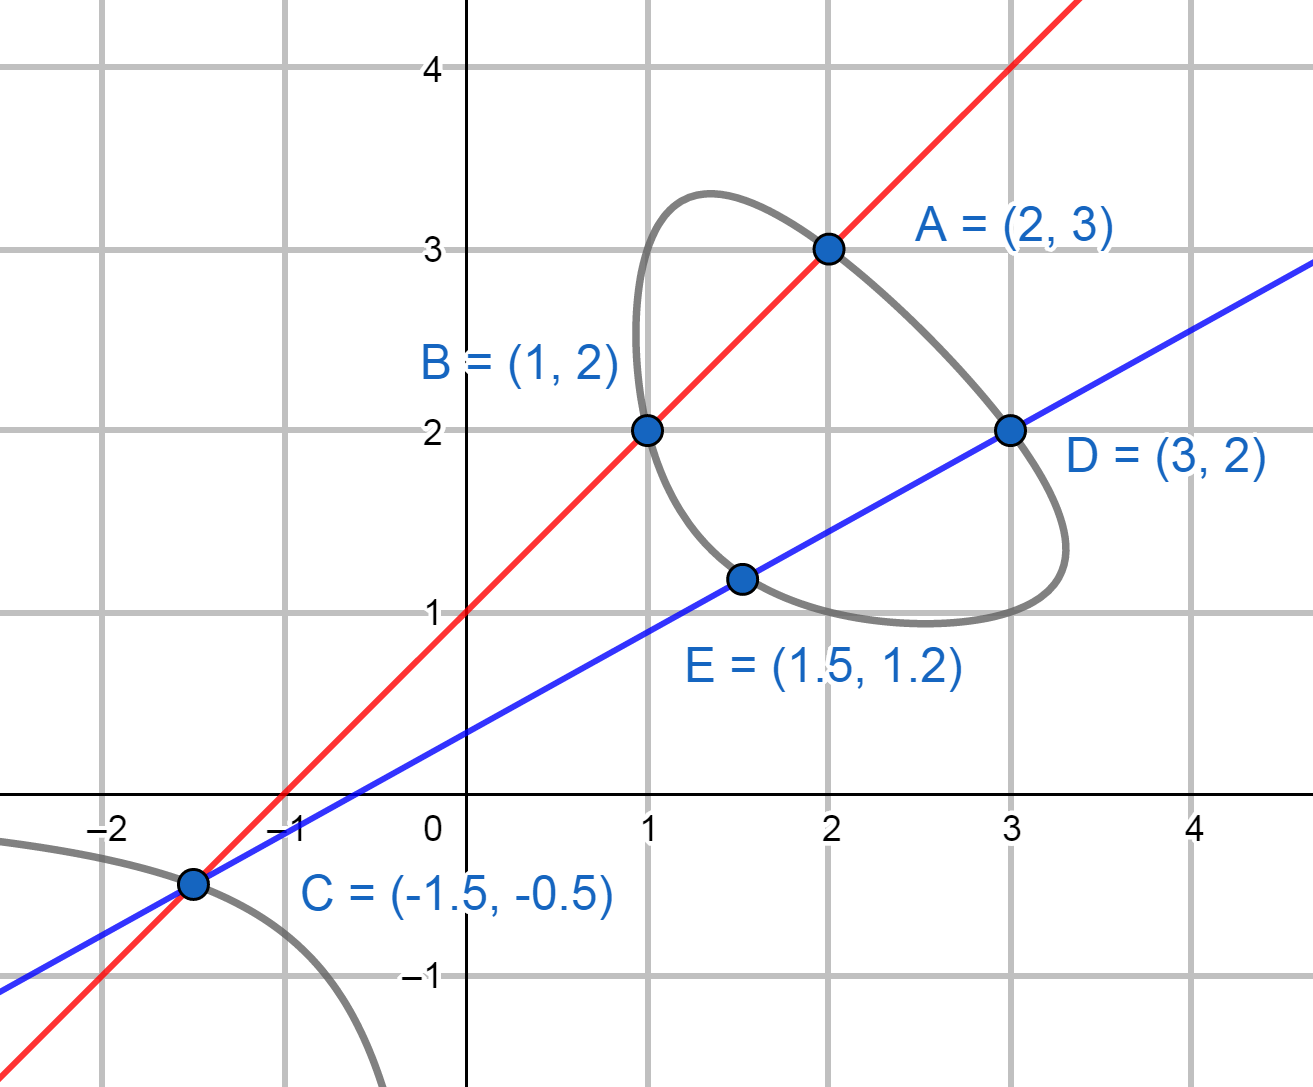
\includegraphics[width=.7\textwidth]{elliptic1}
\end{center}

The equation of the (red) line through $A,B$ is $y=x+1$. Substitute for $y$ in Equation~\ref{eq.elliptic}:
\[
x^2(x+1) + x(x+1)^2 -6x(x+1) +6 =0\,
\]
and simplify:
\[
2x^3 -3x^2 -5x +6 =0\,.
\]
From $A,B$, we know two roots $x=2,x=1$, so we can factor the cubic polynomial as:
\[
(x-2)(x-1)(ax+b)=0\,,
\]
where only the third root is unknown. Multiply the factors and we immediately see that $a$, the coefficient of the cubic term $x^3$, must be $2$, and $2b$, the constant term, must be $6$. Therefore, the third factor is $2x+3$ which gives the third root $x=-\frac{3}{2}$ and $y=x+1=-\disfrac{1}{2}$. This is the point $C=(-\disfrac{3}{2},-\disfrac{1}{2})$ in the graph.

The equation of the second secant (blue) is:
\begin{equation}
y = \frac{5}{9}x + \frac{1}{3}\,.\label{eq.second-secant}
\end{equation}
Substitute for $y$ in Equation~\ref{eq.elliptic}:
\[
x^2\left(\frac{5}{9}x + \frac{1}{3}\right) + x\left(\frac{5}{9}x + \frac{1}{3}\right)^2 -6x\left(\frac{5}{9}x + \frac{1}{3}\right) +6 =0\,,
\]
and simplify:
\[
\frac{70}{81}x^3 - \frac{71}{27}x^2 - \frac{17}{9}x +6 =0\,.
\]
Again, we have two roots $x=3,x=-\disfrac{3}{2}$, so we can factor the cubic polynomial as:
\[
(x-3)(x+\frac{3}{2})(ax+b)=0\,.
\]
Equating the coefficient of the cubic term and equating the constant term give:
\[
\frac{70}{81}x - \frac{4}{3}=0\,,
\]
so:
\[
x=\frac{81}{70}\cdot \frac{4}{3}= \frac{27\cdot 4}{70} = \frac{54}{35}\,.
\]
$y$ can be computed from Equation~\ref{eq.second-secant} and the coordinates of $E$ are:
\[
\left(\frac{54}{35}, \frac{25}{21}\right)\,.
\]
Finally, compute $z$ from Equation~\ref{eq.xy1}:
\[
z=\frac{x+y}{xy-1}=%
\displaystyle\left(\frac{54}{35} + \frac{25}{21}\right)%
 \, / \,%
\displaystyle\left(\frac{54}{35}\frac{25}{21}-1\right)=%
\frac{2009}{615} = \frac{49}{15}\,.
\]

\section{From solutions to the elliptic curve to triangles}

From $x,y,z$, $a,b,c$, the sides of the triangle $\triangle ABC$ can be computed:
\begin{eqnarray*}
a&=&w+v = r(z+y)=(z+y)\\
b&=&u+w= r(x+z)=(x+z)\\
c&=&u+v=r(x+y)=(x+y)\,,
\end{eqnarray*}
since $\displaystyle r=\frac{A}{s}=\frac{6}{6}=1$.

For the solution $A=(2,3)$ of the elliptic curve, the value of $z$ is:
\[
z=\frac{x+y}{xy-1}=\frac{2+3}{2\cdot 3-1}=1\,,
\]
and the sides of the triangle are:
\begin{eqnarray*}
a &=& z+y = 1+3 = 4\\
b &=& x+z = 2+1=3\\
c &=& x+y = 2+3=5\,,
\end{eqnarray*}
the right triangle with $s=A=6$. Computing the sides corresponding to $B$ and $D$ gives the same triangle.

For $E$:
\begin{eqnarray*}
a &=& z+y = \frac{49}{15} + \frac{25}{21} = \frac{156}{35}\\
b &=& x+z = \frac{54}{35} + \frac{49}{15} = \frac{101}{21}\\
c &=& x+y = \frac{54}{35} + \frac{25}{21}  = \frac{41}{15}\,.
\end{eqnarray*}

Let us check the result. The semi-perimeter is:
\[
s=\frac{1}{2}\left(\frac{156}{35} + \frac{101}{21}+\frac{41}{15}\right) = \frac{1}{2}\left(\frac{468+505+287}{105}\right) = \frac{1}{2}\left(\frac{1260}{105}\right)= 6\,,
\]
and the area can be computed using Heron's formula:
\begin{eqnarray*}
A &=& \sqrt{s(s-a)(s-b)(s-c)}\\
&=& \sqrt{6 \left(6-\frac{156}{35}\right) \left(6-\frac{101}{21}\right) \left(6-\frac{41}{15}\right)}\\
&=& \sqrt{6 \cdot \frac{54}{35}\cdot \frac{25}{21} \cdot \frac{49}{15}}\\
&=& \sqrt{\frac{396900}{11025}}\\
&=& \sqrt{36} = 6\,.
\end{eqnarray*}

\section{A proof of Heron's formula}

The triple tangent formula states that if $\phi+\theta+\psi=\pi$ then:
\begin{equation}
\tan\phi+\tan\theta+\tan\psi = \tan\phi\tan\theta\tan\psi\,. \label{eq.triple}
\end{equation}
The proof follows immediately from Equation~\ref{eq.tangent3}:
\begin{eqnarray*}
\tan\psi &=& \tan (\pi-(\phi+\theta))\\
&=& -\tan (\phi+\theta)\\
&=& \frac{\tan\phi+\tan\theta}{\tan\phi\tan\theta-1}\\
\tan\phi\tan\theta\tan\psi-\tan\psi&=& \tan\phi+\tan\theta\\
\tan\phi\tan\theta\tan\psi &=&\tan\phi+\tan\theta+\tan\psi\,.
\end{eqnarray*}
From Equations~\ref{eq.alpha}--\ref{eq.area2}, and $r=A/s$:
\begin{eqnarray*}
A &=& r^2\left(\tan \frac{\alpha}{2}+\tan \frac{\beta}{2}+\tan \frac{\gamma}{2}\right)\\
&=&r^2\left(\tan \frac{\alpha}{2}\tan \frac{\beta}{2}\tan \frac{\gamma}{2}\right)\\
&=&r^2\left(\frac{u}{r}\frac{v}{r}\frac{w}{r}\right)\\
&=&\frac{u\,v\,w}{r}\\
&=&\frac{s}{A}\,u\,v\,w\\
A^2&=&s\,u\,v\,w\,.
\end{eqnarray*}
$s=u+v+w$, so:
\begin{eqnarray*}
s - a &=& (u+v+w) - (w+v) = u\\
s - b &=& (u+v+w) - (u+w) = v\\
s - c &=& (u+v+w) - (u+v) = w\,,
\end{eqnarray*}
and Heron's formula follows:
\begin{eqnarray*}
A^2 &=& s\,u\,v\,w\\
&=& s(s-a)(s-b)(s-c)\\
A &=& \sqrt{s(s-a)(s-b)(s-c)}\,.
\end{eqnarray*}


